\section{Results}
\subsection{Logistic Regression}
Results from the logistic regression are included in figures 
\ref{fig:logistic-basic}, \ref{fig:logistic-confmat}, \ref{fig:logistic-cumul}, 
\ref{fig:logistic-roc}. Figure \ref{fig:logistic-basic} shows the performance of
the logistic regressor without any added sampling techniques, and serves as
a baseline for comparison.
Due to observing varying mean accuracy for the different methods,
cross-validation accuracies were also calculated, and are presented in table
\ref{tab:crossval-logistic}.
All the sampling methods were able to produce perfomances rivaling that of
balanced weighting, but with less stability. The mean accuracy varied between
$~0.60$ to $~0.999$, which is also reflected in the cross-validation scores. 

Figure \ref{fig:forest-performance} shows the analysis results for the random
forest classifier. Based on the cross-validation accuracy scores included
in table \ref{tab:crossvals}, only results obtained when applying random
over-sampling were used for plotting.
Note that the plots are generated from single runs of the code, not averaged
over several.

\begin{figure}[H]
\begin{center}
    \subfloat[]{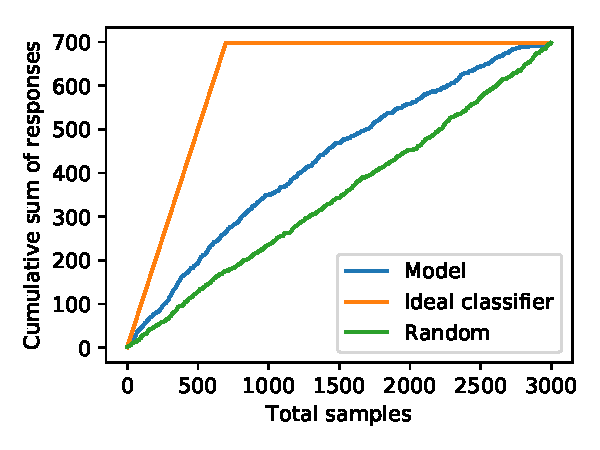
\includegraphics[width=0.4\textwidth, height=0.25\textheight]{figures/logistic_none_cumul}} 
    \subfloat[]{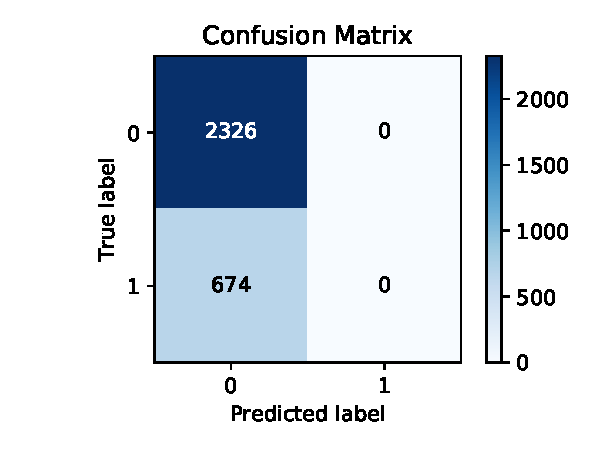
\includegraphics[width=0.4\textwidth, height=0.25\textheight]{figures/logistic_none_confmat}} \\
    \subfloat[]{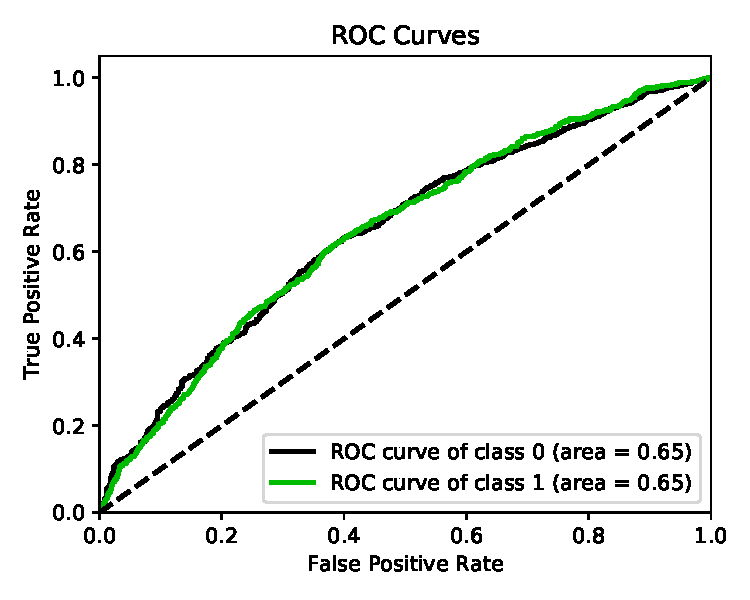
\includegraphics[width=0.5\textwidth]{figures/logistic_none_roc}}
\end{center}
\caption[caption]{Performance analysis for basic logistic regression with no
                    added sampling for balancing.}
\label{fig:logistic-basic}
\end{figure}

\begin{figure}[H]
\begin{center}
    \subfloat[Random oversampling]{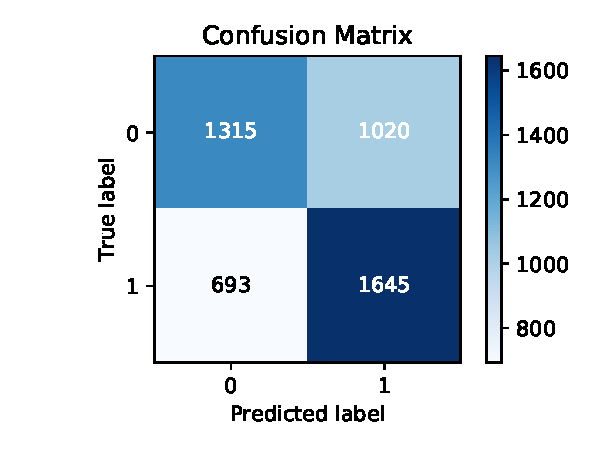
\includegraphics[width=0.4\textwidth, height=0.25\textheight]{figures/logistic_random_oversampling_confmat}} 
    \subfloat[ADASYN]{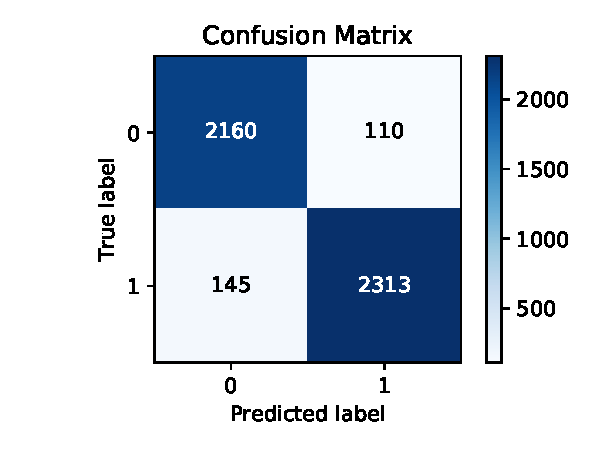
\includegraphics[width=0.4\textwidth, height=0.25\textheight]{figures/logistic_adasyn_confmat}} \\
    \subfloat[SMOTE]{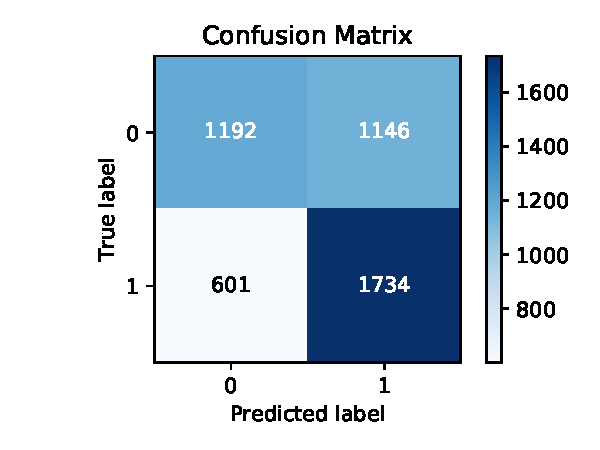
\includegraphics[width=0.4\textwidth, height=0.25\textheight]{figures/logistic_smote_confmat}} 
    \subfloat[Balanced weighting]{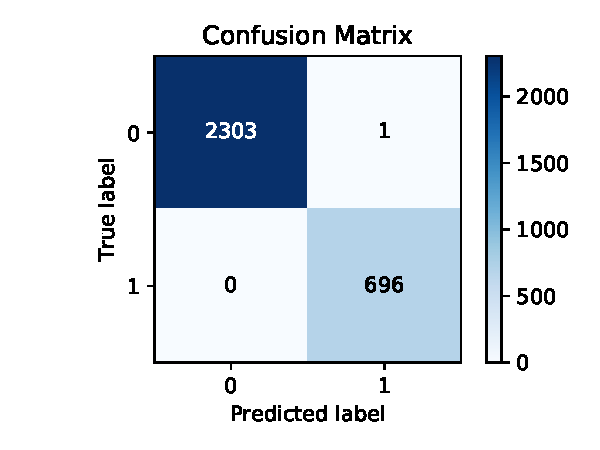
\includegraphics[width=0.4\textwidth, height=0.25\textheight]{figures/logistic_none_balanced_confmat}}
\end{center}
\caption[caption]{Confusion matrices for the logistic regression model using different resampling methods to balance the data set.}
\label{fig:logistic-confmat}
\end{figure}

\begin{figure}[H]
\begin{center}
    \subfloat[Random oversampling]{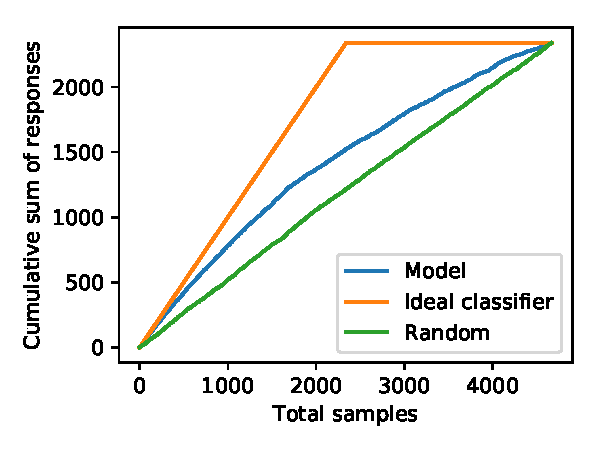
\includegraphics[width=0.4\textwidth, height=0.25\textheight]{figures/logistic_random_oversampling_cumul}} 
    \subfloat[ADASYN]{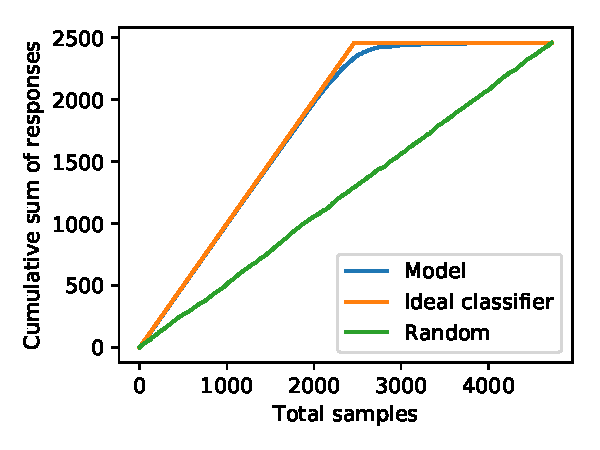
\includegraphics[width=0.4\textwidth, height=0.25\textheight]{figures/logistic_adasyn_cumul}} \\
    \subfloat[SMOTE]{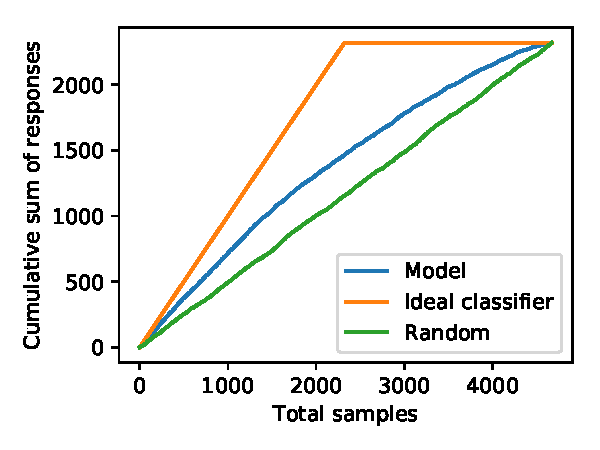
\includegraphics[width=0.4\textwidth, height=0.25\textheight]{figures/logistic_smote_cumul}} 
    \subfloat[Balanced weighting]{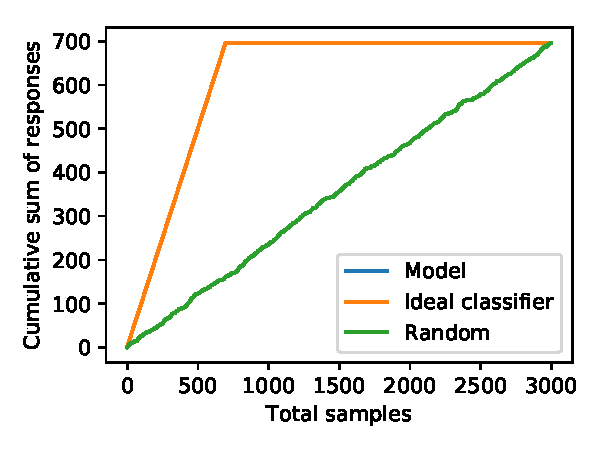
\includegraphics[width=0.4\textwidth, height=0.25\textheight]{figures/logistic_none_balanced_cumul}}
\end{center}
\caption[caption]{Cumulative gain chart for the logistic regression model using different resampling methods to balance the data set.}
\label{fig:logistic-cumul}
\end{figure}

\begin{figure}[H]
\begin{center}
    \subfloat[Random oversampling]{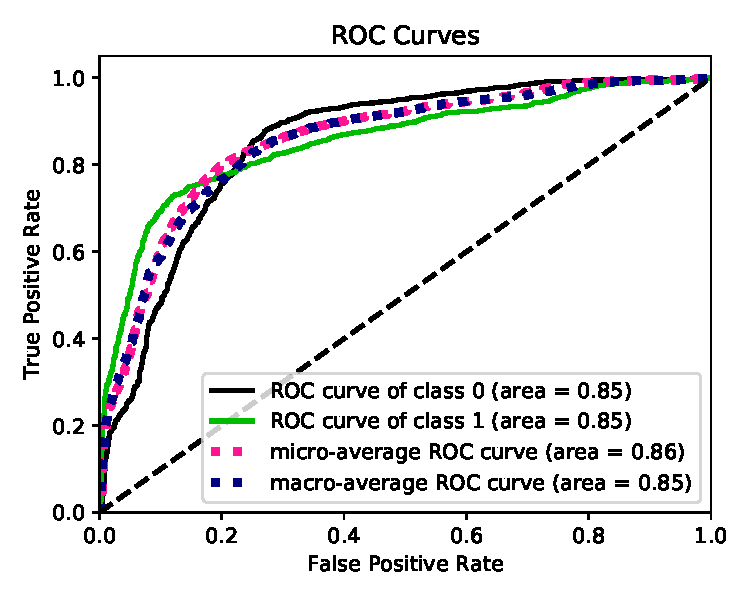
\includegraphics[width=0.4\textwidth, height=0.25\textheight]{figures/logistic_random_oversampling_roc}} 
    \subfloat[ADASYN]{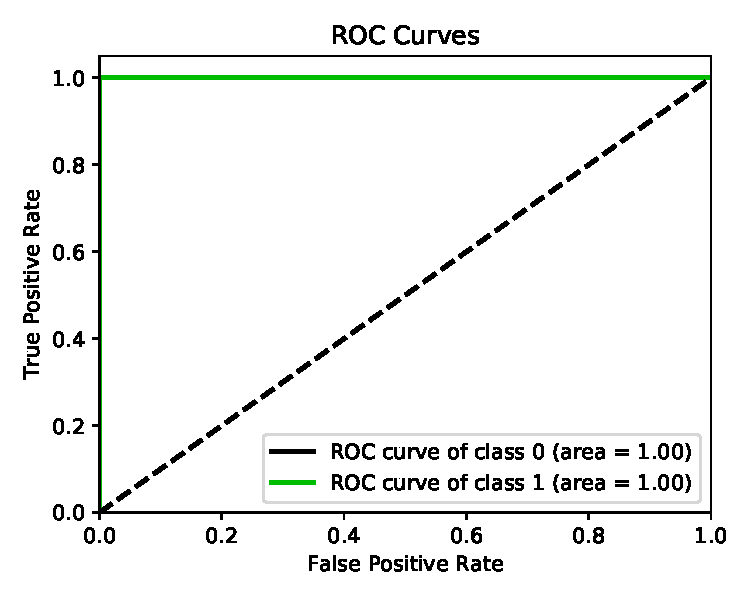
\includegraphics[width=0.4\textwidth, height=0.25\textheight]{figures/logistic_adasyn_roc}} \\
    \subfloat[SMOTE]{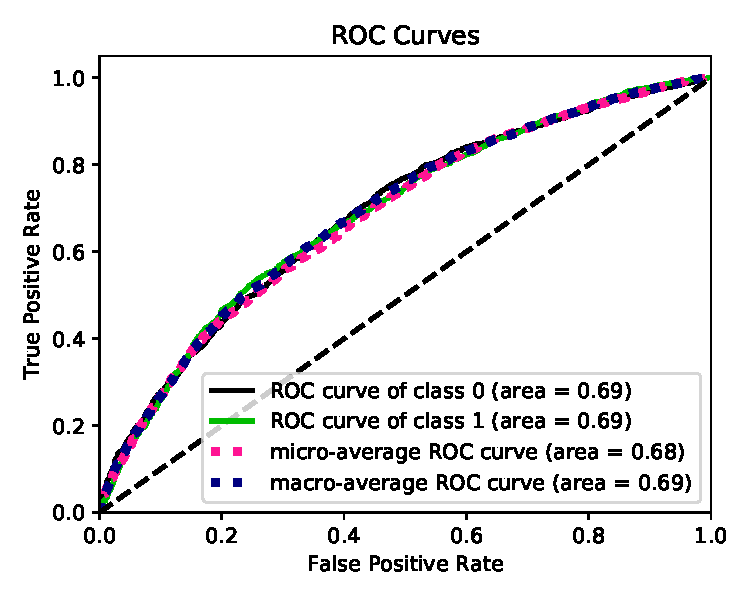
\includegraphics[width=0.4\textwidth, height=0.25\textheight]{figures/logistic_smote_roc}} 
    \subfloat[Balanced weighting]{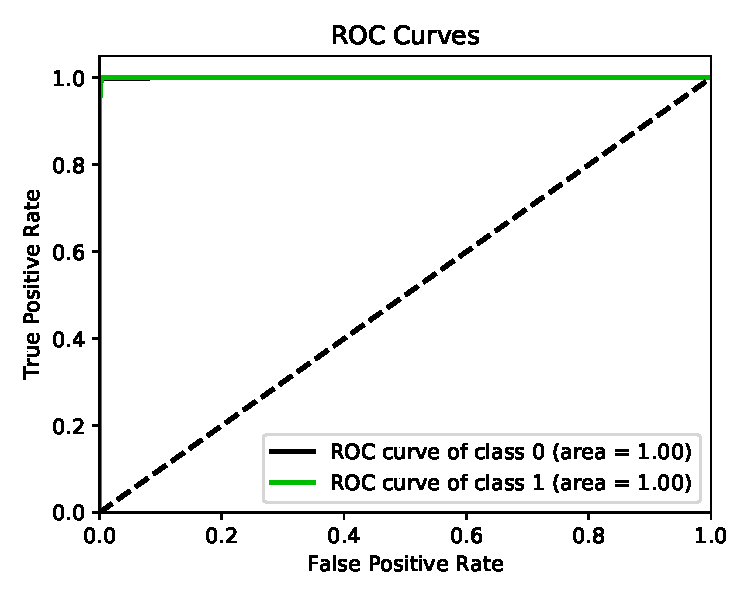
\includegraphics[width=0.4\textwidth, height=0.25\textheight]{figures/logistic_none_balanced_roc}}
\end{center}
\caption[caption]{ROC curves for the logistic regression model using different resampling methods to balance the data set.}
\label{fig:logistic-roc}
\end{figure}

\begin{figure}[H]
\begin{center}
    \subfloat[Cumulative Gain Chart]{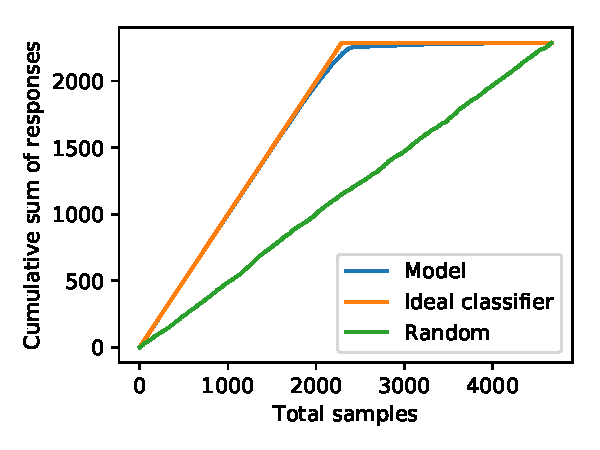
\includegraphics[width=0.4\textwidth, height=0.25\textheight]{figures/forest_random_oversampling_cumul}} 
    \subfloat[Confusion Matrix]{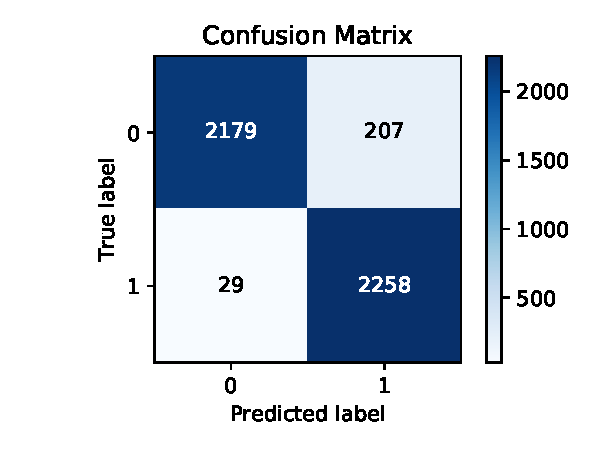
\includegraphics[width=0.4\textwidth, height=0.25\textheight]{figures/forest_random_oversampling_confmat}} \\
    \subfloat[ROC]{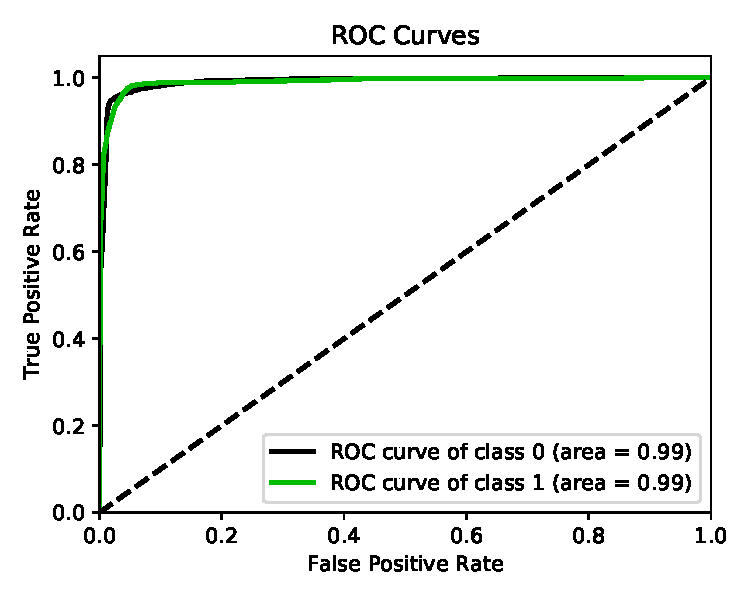
\includegraphics[width=0.5\textwidth]{figures/forest_random_oversampling_roc}}
\end{center}
\caption[caption]{Performance analysis for random forest classification. Only the
    results obtained using random over-sampling are included as they provided the
    best cross-validation accuracy scores (table \ref{tab:crossvals}).}
\label{fig:forest-performance}
\end{figure}

\begin{table}[h]
    \centering
    \caption{Cross-validation accuracies for the different sampling methods
                used with both logistic regression and random forest
                classifier.}
    \label{tab:crossvals}
    \begin{tabular}{l|r|r}
        Sampling method & Logistic & Random Forest \\
        \hline
        None & $0.78 \pm 0.00$ & $0.82 \pm 0.02$ \\
        Random oversampling & $0.85 \pm 0.35$ & $0.94 \pm 0.03$ \\
        SMOTE & $0.84 \pm 0.29$ & $0.84 \pm 0.14$ \\
        ADASYN & $0.95 \pm 0.12$ & $0.82 \pm 0.12$ \\
        Balanced weighting & $1.00 \pm 0.00$ & $0.81 \pm 0.02$ \\
    \end{tabular}
\end{table}

